\newcommand{\placetextbox}[3]{% \placetextbox{<horizontal pos>}{<vertical pos>}{<stuff>}
	\setbox0=\hbox{#3}% Put <stuff> in a box
	\AddToShipoutPictureFG*{% Add <stuff> to current page foreground
		\put(\LenToUnit{#1\paperwidth},\LenToUnit{#2\paperheight}){\vtop{{\null}\makebox[0pt][c]{#3}}}%
	}%
}%

\pagenumbering{gobble}
\fancyhf{}                          % Очищаем текущие значения

\chapter{Теоретическая часть}						

%\placetextbox{0.55}{0.1}{\Huge \textit{This is my text qweqwqweqw.}}%
%  {<width>}
%  [<left handle>,<top handle>]
%  (<leftmargin>,<topmargin>)

\begin{textblock}{10}[0,0](4.5, 10.9)
	\begin{center}
		\Large	Лабораторная работа № 1\\
	\end{center}
\end{textblock}

\begin{textblock}{4}[0,0](5.5, 11.6)
\begin{center}
\Large	Программирование калькулятора\\
\end{center}
\end{textblock}

\begin{textblock}{3}[0,0](12.5, 11.75)
	\pageref{LastPage}
\end{textblock}

\begin{textblock}{3}[0,0](11, 12.3)
	14-В-1
\end{textblock}
	
	
Способность к звуковому поиску, т.е. определение направления на источник звука – важная вещь для биологических организмов, ведь звук может выступать и сигналом опасности и использоваться для поиска жертвы. К  тому же, локализация звука имеет множество инженерных применений, начиная с определения местоположения говорящего, заканчивая автоматическими решениями куда повернуть направленный микрофон, прожектор или камеру.

В настоящее время актуальна проблема разработки систем оценки направления на источник звука. Такие системы могут использоваться как в масштабах определения местонахождения крупных объектов – например, самолетов, подводных лодок, так и в качестве сенсоров для различных устройств, роботов, охранных систем. 

Во то время, когда задача поиска направления на источник звука приобрела свою актуальность, основное внимание было уделено бинауральному методу поиска, как наиболее очевидному и простому. Этот метод основан на нахождении разницы фаз и величины разности амплитуд между записями с двух приемников звука, находящихся в одной плоскости. Однако, не смотря на работоспособность, такой способ имеет ряд недостатков, среди которых малая область поиска, довольно грубый результат и относительно большие габариты установки.

Использование бинаурального метода поиска обуславливалось тем, что человеческий слух и способность воспринимать направление источника звука долгое время присваивались использованию сразу двух ушей. Однако, когда в некоторых экспериментах бинауральный принцип стал недостаточен, начала серьезно изучаться роль ушной раковины в локализации звука. Некоторые эксперименты проводились с источниками звука, лежащими непосредственно на  медиальной вертикальной плоскости и не отклоняющимися куда-либо по горизонтали. Невозможность использования в таких случаях бинаурального метода послужила толчком к усовершенствованию приемника-обработчика и поиску альтернативных методов решения проблемы.

Была сформулирована задача поиска с использованием одного приемника звука. Существующие решения данной задачи, основанные на монауральном принципе, рассмотрены и приняты во внимание . Многие из этих решений обрабатывают сигнал на уровне отсчетов. С другой стороны, известны факты, утверждающие, что, к примеру, механизмы зрительного восприятия человека целостны, при грубо-точном анализе сенсорных данных зрительной системой. В теории активного восприятия (ТАВ) описан метод грубо-точного анализа, который используется при распознавании изображений. 

\chapter{Практическая часть}						

\pagenumbering{arabic}
\setcounter{page}{3}
\rfoot{\thepage}
\fancyfootoffset[L]{-6cm}
\setlength{\footskip}{1.3cm}
\cfoot[EO]{\fontsize{16}{12} \selectfont \textit{Лабораторная работа № 1} }


Способность к звуковому поиску, т.е. определение направления на источник звука – важная вещь для биологических организмов, ведь звук может выступать и сигналом опасности и использоваться для поиска жертвы. К  тому же, локализация звука имеет множество инженерных применений, начиная с определения местоположения говорящего, заканчивая автоматическими решениями куда повернуть направленный микрофон, прожектор или камеру.

В настоящее время актуальна проблема разработки систем оценки направления на источник звука. Такие системы могут использоваться как в масштабах определения местонахождения крупных объектов – например, самолетов, подводных лодок, так и в качестве сенсоров для различных устройств, роботов, охранных систем. 

\begin{figure}[ht] 
	\center
	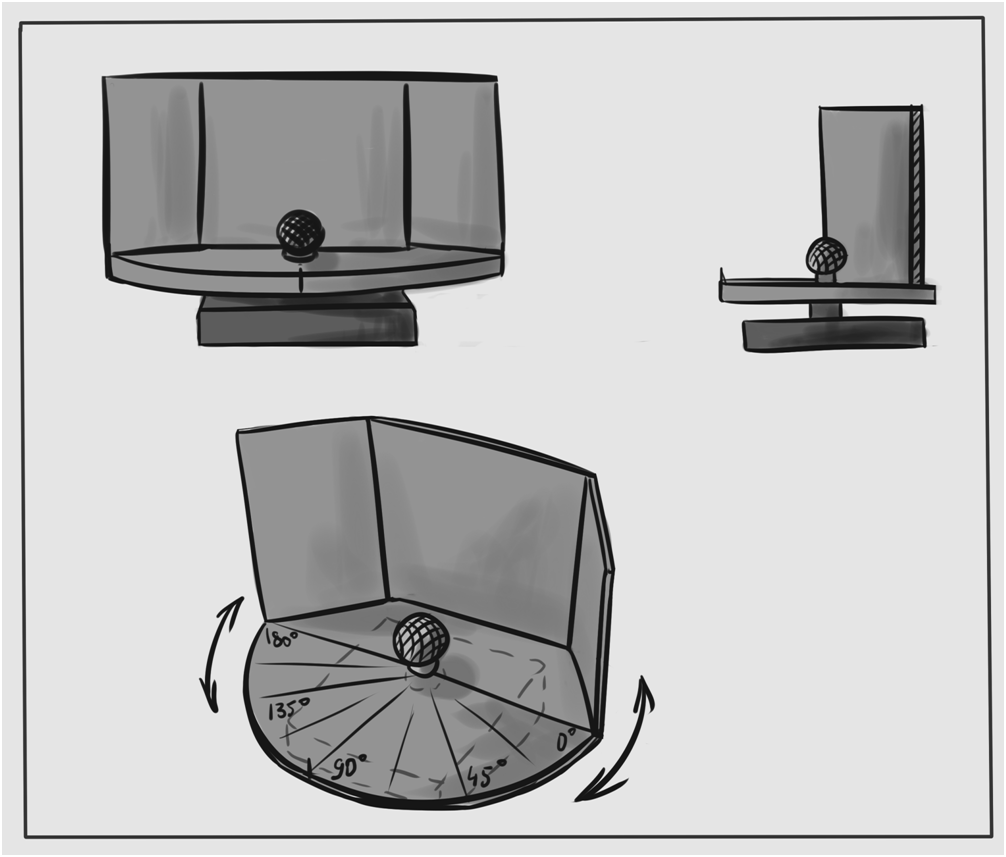
\includegraphics [scale=0.4] {./myimages/pictMaket}
	\caption{Макет установки №1.} 
	\label{img:pictMaket}  
\end{figure}

Во то время, когда задача поиска направления на источник звука приобрела свою актуальность, основное внимание было уделено бинауральному методу поиска, как наиболее очевидному и простому. Этот метод основан на нахождении разницы фаз и величины разности амплитуд между записями с двух приемников звука, находящихся в одной плоскости. Однако, не смотря на работоспособность, такой способ имеет ряд недостатков, среди которых малая область поиска, довольно грубый результат и относительно большие габариты установки.

Использование бинаурального метода поиска обуславливалось тем, что человеческий слух и способность воспринимать направление источника звука долгое время присваивались использованию сразу двух ушей. Однако, когда в некоторых экспериментах бинауральный принцип стал недостаточен, начала серьезно изучаться роль ушной раковины в локализации звука. Некоторые эксперименты проводились с источниками звука, лежащими непосредственно на  медиальной вертикальной плоскости и не отклоняющимися куда-либо по горизонтали. Невозможность использования в таких случаях бинаурального метода послужила толчком к усовершенствованию приемника-обработчика и поиску альтернативных методов решения проблемы.
